\chapter {Arquitetura}

Como ambiente de desenvolvimento integrado (IDE) escolhido foi o eclipse devido ao favorecimento do desenvolvimento rápido com recursos que podem ser integrados através de plugins, além disso sua portabilidade para outras plataformas sem afetar os plugins adicionados favorecendo o desenvolvimento independente da plataforma escolhida pelo desenvolvedor.\\

O Eclipse Java development tools (JDT), fornece plugins que implementam a IDE eclipse servindo com apoio para o desenvolvimento de qualquer aplicativo Java, inclusive plugins para a própria IDE Eclipse.\\

São cinco os componentes que compõem o JDT, e cada componente pode operar com um projeto independente, que são:

	\begin{itemize}
		\item \textbf{APT} fornece plugins que adicionam e fornecem suporte ao processamento de anotações java.
		\item \textbf{Core} é o core da infraestrutura Java da IDE eclipse provendo compiladores, API's modelos definidas em árvores Java, documentação, assitente de código, suporte e formatação de código fonte.
		\item \textbf{Debug} componente de depuração da plataforma sendo definido independente da linguagem utilizada.
		\item \textbf{Text} fornece blocos básicos para editores de texto e textos dentro do eclipse e ainda contribui com o editor de texto padrão do eclipse. \item \textbf{UI} prove toda interface que necessite de iteração com o usuário final, e ainda fornece a manipulação e visualização do código Java na IDE.
	\end{itemize} 
	
\section {Arquitetura}

A arquitetura do analisador a ser implementada utiliza com base os componentes JDT porém de maneira independente da IDE eclipse o qual não é um plugin da IDE mas sim uma ferramente que pode ser utilizada como apoio em qualquer processo de desenvolvimento ou para levantamento de dados sobre a história evolutiva de um software.\\

Esta analisador tem com base para seu funcionamento o uso de visitors\cite{Gamma:1995:DPE:186897} os quais possuem inteligência para verificar a adoção de códigos recentemente adicionados a novas releases da linguagem Java como multicatchs e até mesmo efetuar a pesquisa de código ultrapassados através de padrões pré-definidos para que possam vir a ser melhorados caso o desenvolvedor assim julgue necessário conforme é o caso de vários catchs aninhados que pode ser um potencial caso de se tornar um bloco único de multicatch tornando o código mais elegante, atual e legível.\\

Tais analisador tem como entradas válidas um único arquivo arquivo separado por vírgula (CSV) que possui em seus campos o nome dos projeto, versões e caminho para que cada um seja analisado. Após o input é realizado uma pesquisa em seu diretório \textit{src} o qual contém os códigos Java que compõem o projeto, após todos os arquivos listas é realizado um parse para a construção de árvores de sintáxe abstratas (AST) uma por arquivo e dai é lançando os visitors\cite{Gamma:1995:DPE:186897} com suas respectivas inteligências para pesquisar os padrões previamente definidos os quais são armazenados em uma única coleção de dados que gera um CSV para cada padrão designado e dentro informando onde e em qual versão do projeto fora encontrado.\\
	
\begin{figure}[h]
	\center
	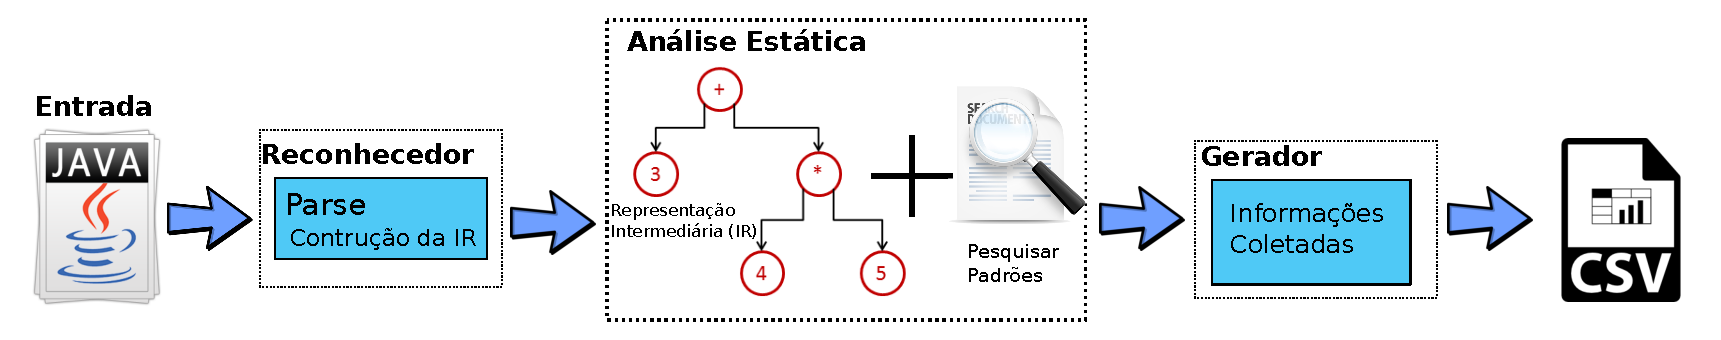
\includegraphics[width=1.0\textwidth]{Imagens/Arquitetura}
	\label{arquiteturaVisitor}
	\caption{Arquitetura geral do software.}
\end{figure}	

\clearpage
\subsection{Visitors}
\begin{figure}[h]
\center
\includegraphics[width=1.0\textwidth]{Imagens/Visitors}
\label{arquiteturaVisitor}
\caption{Organização dos Visitors.}
\end{figure}

Todos os visitors criados para o projeto extendem da classe \textit{Visitor.java} a qual implementa a interface \textit{IVisitor.java}, vale resaltar que a classe \textit{Visitor.java} extende por sua vez de ASTVisitor a qual é fornecida pelo Core do JDT eclipse tendo como método principal utilizado neste projeto o \textbf{boolean visit(Statement node)} o qual recebe como parâmento qualquer Statement descrito na lib JDT, este método é sobrescrito com todo conteúdo necessário para recolher as méticas de acordo com os padrões previamente estabelecidos.\\


\clearpage
\begin{figure}[h]
	\center
	\includegraphics[width=0.8\textwidth]{Imagens/ProjectAnalyser}
	\label{ProjectAnalyser}
	\caption{Project analyser.}
\end{figure}

Este diagrama exibe o coração da aplicação pois é aqui que ocorre a transformação de todo código Java que compõe o projete em árvore sintática para que os visitors\cite{Gamma:1995:DPE:186897} possam pesquisar em seus nós pelos padrões estabelecidos.\\

Um ponto interessante é que o \textit{ProjectAnalyser.java} não tem a responsabilidade de instanciar a lista de IVisitor a qual possui referência pois estas são injetadas usando o padrão de projeto injeção de dependência\textbf{(DI)} o qual aqui faz-se presente através do framework spring que injeta uma lista de \textit{bean} onde cada \textit{bean} representa cada classe de extendida de Visitor descrita anteriormente.\\

\clearpage


\subsection{Inversão de Controle e Injeção de Dependência}
O padrão de projeto inversão de controle \textbf{(IoC)} e injeção de dependência \textbf{(DI)} é utilizado quando deseja-se obter um baixo nível de acoplamento entre módulos que compõem um sistema tornando mais suave ou até mesmo removendo o acoplamento entres módulos para que seja mais fácil evoluir e manter o software. Desta forma a injeção faz-se de maneira configurável através de um arquivo \textit{XML} ou até mesmo uma classe \textit{Java}. Para tal função usaremos o framework Spring devido sua consolidação e popularidade no assunto.\\

Para preparar o ambiente de acordo com as especificações do Spring é necessário definir o contexto da aplicação e para isso é faz-se necessário criar antes de injetar as dependências as configurações iniciais. Dentre as possíveis formas disponibilizadas pelo framework de conceder tal configuração para criação um contexto para aplicação \textit{ApplicationContext} o projeto segue com a criação de um arquivo   \textit{XML} o que concentra as referências necessárias de quais objetos e onde estes serão injetados. O arquivo \textit{XML} criado para tal finalidade é o \textit{'Beans.xml'}. Atualmente na versão 4.1.6 do framework spring é possível utilizar uma classe para fazer o mesmo trabalho do arquivo \textit{XML}. \\

\begin{figure}[h]
	\center
	\includegraphics[width=0.4\textwidth]{Imagens/Beans}
	\label{ProjectAnalyser}
	\caption{Localização Beans.xml.}
\end{figure}
\clearpage

Configuração necessária para o funcionamento da injeção de dependências com Spring conforme explicado na documentação do framework conforme\cite{SPRING_REF}.\\
\begin{lstlisting}
<?xml version="1.0" encoding="UTF-8"?>
	<beans xmlns="http://www.springframework.org/schema/beans"
		xmlns:xsi="http://www.w3.org/2001/XMLSchema-instance" xmlns:context="http://www.springframework.org/schema/context"
		xsi:schemaLocation="http://www.springframework.org/schema/beans 
		http://www.springframework.org/schema/beans/spring-beans-3.0.xsd
		http://www.springframework.org/schema/context 
		http://www.springframework.org/schema/context/spring-context-3.0.xsd">

	</beans>
\end{lstlisting}


O framework trabalha com \textit{beans} onde cada \textit{bean} representa uma classe Java a ser injetada vale ressaltar que essas por simplicidade devem ter o construtor sem parâmetros para que o trabalho possa ocorrer da maneira mais simples, caso seja necessário parâmetros estes sejam passados vias os métodos Sets.\\

Identificação de cada bean no arquivo de configuração \textit{XML}, é atributo \textbf{id} contido na tag \textbf{bean} onde cada deve ser único para que a gerência das dependências ocorra da forma preconizada pelo framework.\\
\begin{lstlisting}
	<bean id="tsVisitor" class="br.unb.cic.sa.visitors.TryStatementVisitor"/>
	<bean id="mdVisitor" class="br.unb.cic.sa.visitors.MethodDeclarationVisitor"/>
	<bean id="typeVisitor" class="br.unb.cic.sa.visitors.TypeDeclarationVisitor"/>
	<bean id="swVisitor" class="br.unb.cic.sa.visitors.SwitchStatementVisitor"/>
	<bean id="enVisitor" class="br.unb.cic.sa.visitors.EnumDeclarationVisitor"/>
	<bean id="ifVisitor" class="br.unb.cic.sa.visitors.IfVisitor"/>
	<bean id="forVisitor" class="br.unb.cic.sa.visitors.ForVisitor"/>
	<bean id="collection" class="br.unb.cic.sa.model.CollectedData"/>
\end{lstlisting}
\clearpage

Todos os beans são injetados na classe \textit{ProjectAnalyser.java} através de uma lista de IVisitor. E desta forma indicamos no \textit{XML} através da tag \textbf{<property name="listVisitors">} onde o atributo \textbf{name} deve conter o mesmo nome que o atributo na classe Java,  neste caso o algo é \textbf{listVisitors} que existe uma lista de IVisitor com este mesmo nome dentro da classe \textit{ProjectAnalyser.java}.\\
\begin{lstlisting}
	<bean id="pa" class="br.unb.cic.sa.ProjectAnalyser">
		<property name="listVisitors">
			<list>
				<ref bean="forVisitor"/>
				<ref bean="ifVisitor"/>
				<ref bean="tsVisitor"/>
				<ref bean="mdVisitor"/>
				<ref bean="typeVisitor"/>
				<ref bean="swVisitor"/>
				<ref bean="enVisitor"/>
			</list>
		</property>
	
	</bean>
\end{lstlisting}


Para concluir com sucesso a injeção faz-se necessário somente indicar em qual classe e em qual local será injetada tal dependêcia, nesse caso a classe é a \textit{ProjectAnalyser.java} e o local é definido pela anotação \textbf{\textit{@Autowired}} logo acima do atributo o qual será injetado.\\

\begin{lstlisting}
	public class ProjectAnalyser... {

		@Autowired
		private List<IVisitor> listVisitors;
		.
		.
		.
	}
\end{lstlisting}
\clearpage

Para finalizar todo ambiente de configuração de injeção de dependência é necessário somente criar uma classe que seja um Singleton\cite{Gamma:1995:DPE:186897} conforme cita Gamma e amigos e faz-se necessária conforme indica a documentação\cite{SPRING_REF}, para ter o controle de que exista somente um único ambiente de injeção.\\
Tal padrão que controla a quantidade de instâncias dos objetos se faz presente através da classe \textit{CDI.java} qual
\begin{lstlisting}
	public class CDI {
	
		private static CDI instance;
		private ApplicationContext ctx;
		
		private CDI(){ 
			ctx = new ClassPathXmlApplicationContext("Beans.xml");
		}
		
		public static CDI Instance(){
			if(instance == null)
				instance = new CDI();
		
			return instance;
		}
		
		public ApplicationContext getContextCdi(){
			return ctx;
		}
	}
\end{lstlisting}

As bibliotecas necessárias para que o ambiente de injeção de dependência ocorra na linguagem \textit{Java} são:
\begin{itemize}
	\item spring-aop-4.1.6.RELEASE.jar
	\item spring-beans-4.1.6.RELEASE.jar
	\item spring-context-4.1.6.RELEASE.jar
	\item spring-core-4.1.6.RELEASE.jar
	\item spring-expression-4.1.6.RELEASE.jar
\end{itemize}
\clearpage

As quais devem ser adicionadas ao diretório \textbf{lib} do projeto tendo suas referências atualizadas, conforme ilustrada da figura abaixo.\\
\begin{figure}[h]
	\center
	\includegraphics[width=0.4\textwidth]{Imagens/libsSpring}
	\label{ProjectAnalyser}
	\caption{Libs Spring necessárias para CDI.}
\end{figure}

